\section{Related Work} % (fold)
\label{sec:related_work}

\subsection{\acs{atm}} % (fold)
\label{sub:atm}
For the sake of completeness, we will briefly look at \acs{atm}. \ac{atm} is a legacy protocol that has been used by operators to carry traffic over the internet backbone since the 1990s. Where as Ethernet and \ac{ip} are developed as packet-routing connection-less protocols, \ac{atm} is a cell-switched connection-oriented protocol. This poses a number of problems when trying to transport \ac{ip} over \ac{atm}. First, the variable length of the packets don't map efficiently to the fixed size cells of \ac{atm}. Drops of a single cell would cause the entire frame to become unusable. Then there is the added overhead of encapsulating \ac{ip} over \ac{atm}, which causes inefficient use of the network resources when compared to running an all \ac{ip} network. Finally, the \ac{qos} features of \ac{atm} are left unused \cite{atm}. These problems are some of the reasons that operators have moved away from \ac{atm} based backbones, to all \ac{ip} ones.

% subsection atm (end)



\subsection{\acs{spb}} % (fold)
\label{sub:spb}

\ac{spb} is an evolution of the original \acs{ieee} 802.1Q \ac{vlan} standard. \ac{vlan} tags have been in use in the networking world for a long time and provide separation in campus networks. However, when \ac{vlan}-tagging was done at the customer network, the carrier couldn't separate the traffic from different customers anymore. This resulted in 802.1Qad or Q-in-Q which added an S-\ac{vlan} tag to separate the client \acp{vlan} from the \ac{sp} \acp{vlan} in the backbone. This was usable for the Metro Ethernet networks for a while but when \acp{sp} started providing this services to more and more customers, their backbone switches could not keep up with the clients \ac{mac} addresses.

To provide the required scalability with regard to \acp{mac} in the backbone, \ac{pbb} (802.1Qay or \ac{mac}-in-\ac{mac}) was introduced. It encapsulates the whole Ethernet frame on the edge of the carrier network and forwards the frame based on the Backbone-\ac{mac} of the egress \ac{pe}. It also separated client \acp{vpn} using a \ac{isid}, which with 24 bits is able to supply the carrier with 16 million separate networks. The downside of \ac{pbb} remained one that is common to all Layer 2 forwarding protocols: the possibility of loops. Preventing them requires \ac{stp} which will disable links to get a loop-free network. Disadvantages of \ac{stp} include the relatively long convergence time and inefficient use of resources due to the disabled links. This has been solved by using \acs{isis} as a routing protocol to discover the network topology. After which each \ac{pe} creates a \acp{spt} originating from each edge device to every other \ac{pe}. This is called \ac{spb} or 802.1aq.

\ac{spb} benefits from the maturity of the Ethernet protocol by reusing protocols for \ac{oam} and \ac{pm}. This allows for fast error detection and extensive troubleshooting tools by using the \ac{ieee} 802.1ag and \ac{itut} Y.1731 standards respectively. The \ac{isis} implementation has also been adapted to rapidly detect errors however, no fast recovery function has been defined, besides complete \ac{isis} reconvergence. This would result in a traffic impact of several hundreds of milliseconds in large networks \cite{spb-nanog}. 

However, due to its Ethernet \acs{stp} forwarding-based nature it lacks \ac{te} features. The paths that the \ac{vpn} traffic takes are not explicitly configureable and provide limited scalability due to limited amounts of available paths (or trees in this case). As such, operators can not define constraints or explicit paths to take over the network to distribute traffic in an efficient manner. The lack of available paths also negatively affects its \ac{ecmp} functionalities. However, future, additional algorithms with multiple paths maybe introduced using extensible \ac{ect} algorithms \cite{rfc6329}.

\begin{figure}[!h]
	\centering
	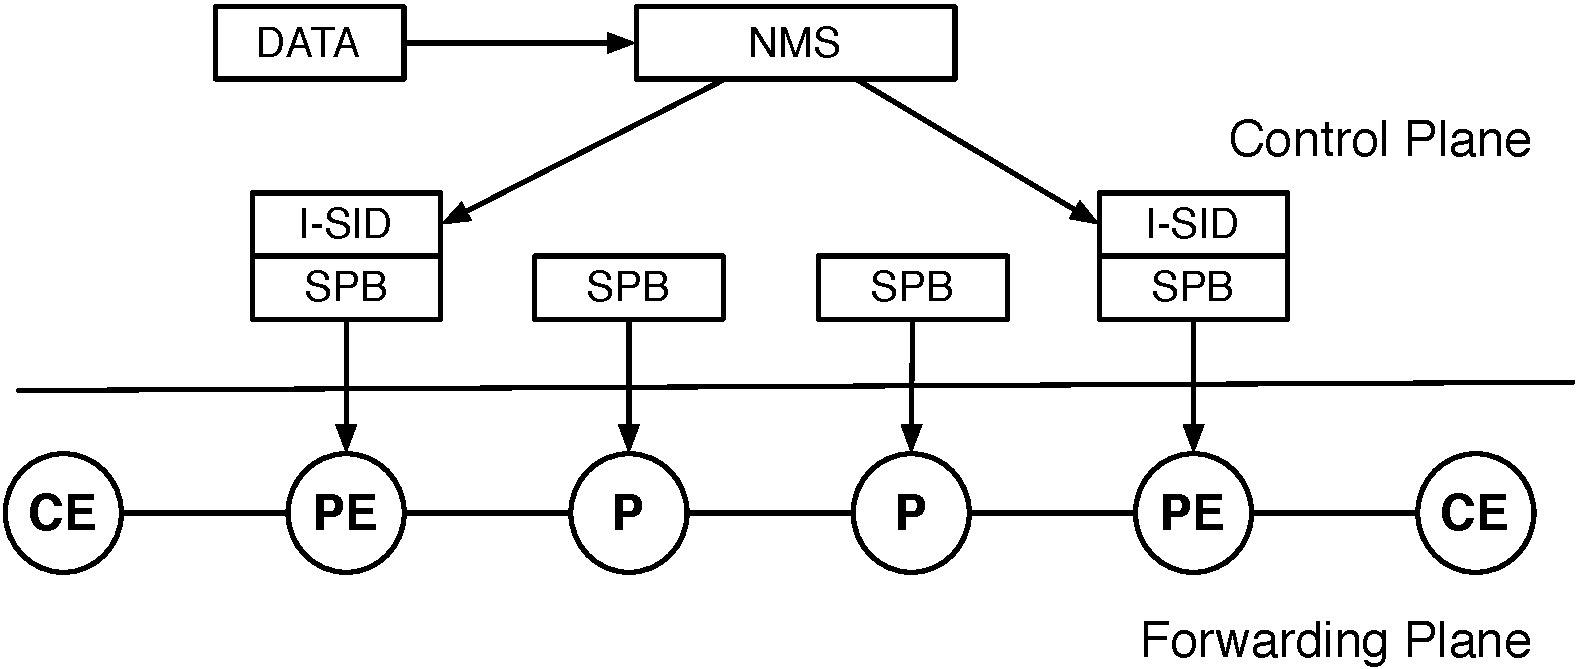
\includegraphics[width=10cm]{./includes/spb-stack.pdf}
	\caption{Provisioning a \ac{dvpn} using \ac{spb}.}
	\label{fig:spb-stack}
\end{figure}

Provided that \ac{isis} has been configured on all provider devices, Figure~\ref{fig:spb-stack} illustrates the interfaces needed to provision a \ac{dvpn} in \ac{spb}. It excels in its simplicity by providing `single-point provisioning'. This means that the \ac{nms} only needs to add the member \ac{ce} port to a certain \ac{dvpn} \ac{isid}, after which the \ac{pe} floods this binding through the \ac{isis} network and other \acp{pe} sharing this \ac{isid} will install the path towards the ingress \ac{pe}. The rate limiting of the \ac{ce} ports is a vendor-specific feature however, and may vary per hardware platform.

The simplicity of the architecture comes at a cost. The protocols has:
\begin{itemize}
	\item limited explicit or constraints-based routing, meaning few \ac{te} features,
	\item limited \ac{ecmp} functionality due to the infancy of the standard to support it, and
	\item because failure recovery depends on \ac{isis} reconvergence, no fast failover.
\end{itemize}

These limitations are being worked on by the community, e.g.\ IEEE 802.1Qbp which provides extensive \ac{ecmp} functions. And since the technology has only been officially standardized since March 2012, it will also need to mature before it is suitable for carrier implementations.  

%Because of the shortcomings of \ac{spb} with regards to the use-case set forth in Section~\ref{sec:dvpns}, we will omit this technology in our comparison. Instead we will focus on comparing the \ac{mpls} setup from Section~\ref{ssub:mpls} with the \acs{sdn}/OpenFlow architecture as designed in Section~\ref{sub:openflow}.

% subsection spb (end)

% section related_work (end)
